%% thesis.tex 2014/04/11
%
% Based on sample files of unknown authorship.
%
% The Current Maintainer of this work is Paul Vojta.





\documentclass{ucbthesis}
\usepackage{biblatex}
\usepackage{rotating} % provides sidewaystable and sidewaysfigure



\usepackage[utf8]{inputenc}
\usepackage{mathrsfs} \usepackage[left=1.25in,top=1.25in,right=1.25in,bottom=1.25in,head=1.25in]{geometry}
\usepackage{amsfonts,amsmath,amssymb,amsthm}
\usepackage{verbatim,float,url,enumerate}
\usepackage{mathtools}
\usepackage{MnSymbol}
\makeatletter
\let\c@lofdepth\relax
\let\c@lotdepth\relax
\makeatother
\usepackage{graphicx,subfigure,psfrag}
\usepackage{environ}
\usepackage{hyperref}
\usepackage{pifont}
\usepackage{xcolor}
% \usepackage{natbib}
\usepackage{graphicx}
\usepackage{color}

\usepackage{booktabs} % boldline 
\usepackage{tikz}
\usetikzlibrary{chains,scopes,positioning,backgrounds,shapes,fit,shadows,calc,arrows.meta}

\newtheorem{algorithm}{Algorithm}
\newtheorem{theorem}{Theorem}
\newtheorem{lemma}{Lemma}
\newtheorem{corollary}{Corollary}
\theoremstyle{remark}
\newtheorem{remark}{Remark}
\theoremstyle{definition}
\newtheorem{definition}{Definition}

\newcommand{\argmin}{\mathop{\mathrm{argmin}}}
\newcommand{\argmax}{\mathop{\mathrm{argmax}}}
\newcommand{\minimize}{\mathop{\mathrm{minimize}}}
\newcommand{\maximize}{\mathop{\mathrm{maximize}}}
\newcommand{\st}{\mathop{\mathrm{subject\,\,to}}}
\newcommand{\dist}{\mathop{\mathrm{dist}}}
\newcommand\iidsim{\stackrel{\mathclap{iid}}{\sim}}
\newcommand\independ{\perp \!\!\! \perp}

\newcommand{\reals}{\mathbb R}
\newcommand{\prox}{\operatorname{prox}}
\newcommand{\dom}{\operatorname{dom}}
\def\R{\mathbb{R}}
\def\E{\mathbb{E}}
\def\P{\mathbb{P}}
\def\A{\mathscr{A}}
\def\B{\mathscr{B}}
\def\L{\mathscr{L}}
\def\N{\mathcal{N}}
\def\X{\mathscr{X}}
\def\Y{\mathscr{Y}}
\def\d{\mathrm{d}}
\def\Kr{\mathrm{Kr}}
\def\K{\mathrm{K}}
\def\Cov{\mathrm{Cov}}
\def\Dir{\mathrm{Dir}}
\def\Var{\mathrm{Var}}
\def\half{\frac{1}{2}}
\def\sign{\mathrm{sign}}
\def\supp{\mathrm{supp}}
\def\th{\mathrm{th}}
\def\tr{\mathrm{tr}}
\def\dim{\mathrm{dim}}
\def\hbeta{\hat{\beta}}


% To compile this file, run "latex thesis", then "biber thesis"
% (or "bibtex thesis", if the output from latex asks for that instead),
% and then "latex thesis" (without the quotes in each case).

% Double spacing, if you want it.  Do not use for the final copy.
% \def\dsp{\def\baselinestretch{2.0}\large\normalsize}
% \dsp

% If the Grad. Division insists that the first paragraph of a section
% be indented (like the others), then include this line:
% \usepackage{indentfirst}

\addtolength{\abovecaptionskip}{\baselineskip}



\bibliography{references}

\hyphenation{mar-gin-al-ia}
\hyphenation{bra-va-do}

\begin{document}
	
	% Declarations for Front Matter
	
	\title{Statistical Learning Theory}
	\author{Oscar Zhang}
	\degreesemester{Spring}
	\degreeyear{2022}
	\degree{}
	\chair{}
	\othermembers{}
	% For a co-chair who is subordinate to the \chair listed above
	% \cochair{Professor Benedict Francis Pope}
	% For two co-chairs of equal standing (do not use \chair with this one)
	% \cochairs{Professor Richard Francis Sony}{Professor Benedict Francis Pope}
	\numberofmembers{3}
	% Previous degrees are no longer to be listed on the title page.
	% \prevdegrees{B.A. (University of Northern South Dakota at Hoople) 1978 \\
	%   M.S. (Ed's School of Quantum Mechanics and Muffler Repair) 1989}
	\field{Mathematics}
	% Designated Emphasis -- this is optional, and rare
	% \emphasis{Colloidal Telemetry}
	% This is optional, and rare
	% \jointinstitution{University of Western Maryland}
	% This is optional (default is Berkeley)
	% \campus{Berkeley}
	
	% For a masters thesis, replace the above \documentclass line with
	% \documentclass[masters]{ucbthesis}
	% This affects the title and approval pages, which by default calls this
	% document a "dissertation", not a "thesis".
	
	\maketitle
	% Delete (or comment out) the \approvalpage line for the final version.
	\approvalpage
	\copyrightpage
	
	% (This file is included by thesis.tex; you do not latex it by itself.)

\begin{abstract}

% The text of the abstract goes here.  If you need to use a \section
% command you will need to use \section*, \subsection*, etc. so that
% you don't get any numbering.  You probably won't be using any of
% these commands in the abstract anyway.

This doc is a summary of statistics and basic machine learning theory.

\end{abstract}

	
	\begin{frontmatter}
		
		\begin{dedication}
			\null\vfil
			\begin{center}
				
			\end{center}
			\vfil\null
		\end{dedication}
		
		% You can delete the \clearpage lines if you don't want these to start on
		% separate pages.
		
		\tableofcontents
		\clearpage
		\listoffigures
		\clearpage
		\listoftables
		
		\begin{acknowledgements}
			Bovinely invasive brag; cerulean forebearance.
			Washable an acre. To canned, silence in foreign.
			Be a popularly. A as midnight transcript alike.
			To by recollection bleeding. That calf are infant. In clause.
			Buckaroo loquaciousness?  Aristotelian!
			Masterpiece as devoted. My primal the narcotic. For cine?
			In the glitter. For so talented. Which is confines cocoa accomplished.
			Or obstructive, or purposeful.
			And exposition? Of go. No upstairs do fingering.
			
		\end{acknowledgements}
		
	\end{frontmatter}
	
	\pagestyle{headings}
	
	% (Optional) \part{First Part}
	
	\chapter{Introduction}

\section{Problem Definition}
Generally, we denote a data set as $X$ and label as $Y$.
$$\textbf{X}=
\begin{bmatrix}
	x_{11} & \dots & x_{1p} \\
	x_{21} & \dots & x_{2p} \\
	\vdots & \ddots& \vdots \\
	x_{n1} & \dots &x_{np}
\end{bmatrix} 
=
\begin{bmatrix}
	\Vec{x_1}\\
	\vdots \\
	\Vec{x_n}
\end{bmatrix}
$$
\subsection{Machine Learning Problem}
$$\text{Unsupervised Learning}
\begin{cases} 
	\text{Dimension Reduction} (\vec{x_i}\in\R^p\mapsto \vec{z_i}\in\R^q, p>q) & \begin{cases}
		\text{linear mapping} \\
		\text{non-linear mapping}
	\end{cases} \\
	\text{Clustering} & \\
\end{cases}
$$

$$
\text{supervised Learning}
\begin{cases}
	\text{classification}\begin{cases}
		y:output\in \{1,\dots,k\}\\
		x:input
	\end{cases}\\
	\text{regression}\\
	\text{Ranking } \vec{x_1},\dots,\vec{x_n}\mapsto y <\text{Isotonic Regression}>
\end{cases}
$$

\subsection{Method}
	\subsubsection{Frequentist View}
	The frequentist approach views the model parameters as unknown constants and estimates them by matching the model to the training data using an approximate metric.
	
	$\{(\vec{x_i},y_i)\}_{i=1}^n,\quad y\in\R, \quad \vec{x_i}\in \R^p$ 
	$\quad \Rightarrow \quad \text{least sqr: }\sum\limits_{i=1}^{n}(y_i - \vec{x_i}^Ta)^2$\\
	$$\text{MLE: } y_i\stackrel{i.i.d}{\sim}N(x^Ta,\sigma^2)=\frac{1}{(2\pi)^{1/2}\sigma}\left( -\frac{(y_i - x_i^Ta)^2}{2\sigma^2}\right)$$
	
	\subsubsection{Bayesian}
	$$y\sim N(x^Ta, \sigma^2) \quad \text{prior distribution:} a\sim N(0, \lambda^2)$$
	$$\Rightarrow P(a|x), \text{ for posterior probability}$$
	\begin{enumerate}[(1)]
		\item $\prod_{i=1}^{n}P(x_i|a)\Leftrightarrow-\sum_{i=1}^{n}\log P(x_i|a)$
		\item $a\sim P(a|\lambda), \quad P(a|x)=\frac{P(x|a)P(a|\lambda)}{P(x)}\Rightarrow $ \begin{enumerate}[i]
			\item $\max P(a|x)$
			\item sample
		\end{enumerate}
	\end{enumerate}


\subsection{Parameterize}
In a parametrical model, the number of parameters is fixed once and, for all, irrespective of the number of training data.

\subsection{Non-Parameter}
The number of parameter grows as the number training data increases. For example, the \textit{logistic regression} and \textit{nearest neighbor} method.
\paragraph{Logistic Regression}
$$P(y=1|x,a)=\frac{1}{1+\exp(-x^Ta)}$$
\paragraph{Nearest Neighbor}
\leavevmode
Put an KNN pic.

	\chapter{Probability}

\section{Sample Space and Events}
\leavevmode
The sample space $\Omega$ is the set of possible outcomes of an experiment $w\in \Omega$ which is called \textbf{sample outcome} (realization or elements). Subsets of $\Omega$ are called \textbf{Events}. Given an event $A$, let $A^C=\{w\in Omega,w\notin A\}$ denote \textbf{the complement of A}.
\subsubsection{monotonicity}
\begin{enumerate}
	\item A sequence of sets $A_1,\dots,A_n,\dots$ is \textbf{monotonic increasing} if $A_1\subset A_2 \subset A_3\subset\cdots$, we define $\lim\limits_{n\to\infty}A_n=\mathop{\bigcup}\limits_{1=1}^{\infty}A_i$
	\item  A sequence of sets $A_1,\dots,A_n,\dots$ is \textbf{monotonic decreasing} if $A_1\supset A_2 \supset A_3\supset \cdots$, we define $\lim\limits_{n\to\infty}A_n=\mathop{\bigcap}\limits_{i=1}^{\infty}A_i$
\end{enumerate}

	\paragraph{Ex 1.}
		$\Omega = \R, A_i=\left[0, 1/i\right), \text{for }i=1,2,...$
		
		$$\bigcup_{i=1}^{\infty}A_i=\left[0,1\right),\quad \bigcap_{i=1}^{\infty}A_i=\{0\}$$
		

\section{$\sigma$-Field and Measures}

\begin{definition}
	Let $\mathscr{A}$ be a collection of subsets of a sample space $\Omega$. $\A$ is called \textbf{$\sigma$-field} (or $\sigma$-algebra) iff it has the following properties:
	\begin{enumerate}[(i)]
		\item $\emptyset \in \A$
		\item If $A\in \A \Rightarrow A^C \in \A$
		\item if $A_i \in \A\Rightarrow \mathop{\bigcap}\limits_{i=1}^{\infty}A_i\in \A	$ 
	\end{enumerate}
	A pair $(\Omega, \A)$ is called a \textbf{measurable space}. The element of $\A$ are called \textbf{measurable sets}.
\end{definition}
Therefore, $\emptyset \in \A;\quad \mathop{\bigcap}_{i=1}^{\infty} A_i\in \A$.

\paragraph{Ex 2.} Let $A$ be a non-empty proper subset of $\Omega$ ($A\neq \emptyset,A\neq\Omega$). The minimum $\sigma$-field is $\{\emptyset,\Omega, A, A^C\}$

\paragraph{Ex 3.} $\Omega=\R$, $\A$ is the smallest $\sigma$-field that contains all the finite open subsets of $\R$, which is called the \textbf{Borel $\sigma$-field} $\B(\R)$.


\begin{definition}
	Let $(\Omega, \A)$ be a measurable space. A set function $v$ defined in $\A$ is called a \textbf{measure} (or belief) iff
	\begin{enumerate}[(i)]
		\item $0\leq v(A)\leq \infty$ for any $A\in \A$
		\item $v(\emptyset) = 0$
		\item if $A_i\in \A$ and $A_i$ are disjointed ($A_i\cap A_j=\emptyset$, if $i\neq j$) then $v(\mathop{\bigcup}\limits_{i=1}^{\infty}A_i)=\sum\limits_{i=1}^{\infty}v(A_i)$
	\end{enumerate}
Triple $(\Omega, \A,v)$ is called a \textbf{measure space}. If $v(\Omega)=1$, the $v$ is called a \textbf{probability measure} and denote it by $P$. Moreover, $(\Omega, \A, P)$ is called a probability space.
\end{definition}


	\paragraph{Ex 4.(Counting Measure)} Let $\Omega$ be a sample space, $\A$ is the collection of all subsets and $v(A)$ is the number of elements in $A$.
	
	\paragraph{Ex 5. Lebesgue Measure} $(\R,\B)\longmapsto m(\left[a,b\right])=b-a$
\subsubsection{Properties}
	\begin{enumerate}[(i.)]
		\item $A\subset B \Rightarrow P(A)\leq P(B)$. (Monotonicity)
		\begin{lemma}
			For any events $A$ and $B$, $P(A\cup B)=P(A) + P(B) - P(A\cap B)$
		\end{lemma}
		\item If $A_n\to A, P(A_n)\to P(A)$, $n\to \infty$ (Continuity)
		\begin{proof}
			Suppose $A_1\subset\A_2\subset\cdots$, let $A=\lim\limits_{n\to\infty}A_n=\mathop{\bigcup}\limits_{i=1}^{\infty}A_i$\\
			\begin{align*}
				B_1 &= A_1 \\
				B_2 &= \{w\in\Omega,w\in A_2,w\notin A_1\}\\
				B_2 &= \{w\in\Omega,w\in A_3,w\notin A_1,A_2\}\\
				\dots &
			\end{align*}
			$$\Rightarrow A_n = \mathop{\bigcup}\limits_{i=1}^{n}A_i = \mathop{\bigcup}\limits_{i=1}^{n}B_i$$
			$$ P(A_n)=P\left(\mathop{\bigcup}\limits_{i=1}^{n}B_i\right)=\sum\limits_{i=1}^{\infty}P(B_i)=P\left(\sum\limits_{i=1}^{\infty}B_i\right)=P(A)$$
			
			$$\tilde{A_1}\Leftarrow A_1\cap A,\quad \tilde{A_2}\Leftarrow(A_1\cup A_2)\cap A, \dots, \tilde{A_n}=\left(\mathop{\bigcup}\limits_{i=1}^{n} A_i\right)\cap A$$
		\end{proof}
	\end{enumerate}

\section{Independent Events}

\begin{definition}[Independence]
	Two events $A$ and $B$ are \textbf{independent} if 
	$$P(A,B)\triangleeq P(A\cap B)=P(A)P(B) \quad (A\upmodels B)$$
	For a set of events $\{A_i,i\in I\}$, $A_i$ are independent if $P(\mathop{\bigcap\limits_{i\in I}}A_i)=\prod\limits_{i\in I} P(A_i)$ for every finite subset $i$ in $I$.
\end{definition}


\begin{definition}[Conditional Probability]
	Assume $P(B)>0$, conditional probability of $A$ given $B$ is:
	$$P(A|B)=\frac{P(AB)}{P(B)}$$
\end{definition}

\begin{lemma}
	If $A\upmodels B$, then $P(A|B)=P(A)$.
\end{lemma}

\subsection{Bayes' Theorem}

\begin{theorem}[The Law of Total Probability]
	Let $A_1, A_2, \dots, A_n$ be a partition of $\Omega$, which means:
	\begin{enumerate}[(1)]
		\item $\mathop{\bigcup}\limits_{i=1}^{k}A_i=\Omega$
		\item $A_i\cap A_j=\emptyset$ for $i\neq j$
	\end{enumerate}
for any event $B$, we have
$$P(B) = \sum_{i=1}^{k}P(B|A_i)P(A_i)$$
\end{theorem}

\begin{theorem}[Bayes' Theorem]
	Let $A_1, A_2, \dots, A_n$ be a partition of $\Omega$, such that $P(A_i)>0$. If $P(B)>0$, then
	$$P(A_i|B) = \frac{P(B|A_i)P(A_i)}{\sum_{j=1}^{k}P(B|A_j)P(A_j)}$$
\end{theorem}
	\chapter{Random Variables}

\section{Random Variable}
\begin{definition}
	In a probability space $P(\Omega, \A, P)$, a random variable is measurable map which means for each $x$, we have $\{w:X(x)\leq x\}\in \A$ where $X:\Omega\to \R$ that assigns a real number $X(w)$ to each outcome $w$.
\end{definition}

\begin{definition}
	For random variable $x$, $A\subset \R$, $X^{-1}(A)=\{w\in\Omega, X(w)\in A\}$.Let
	$$P(X\in A)\triangleeq P(X^{-1}(A))=P(\{w\in\Omega, X(w)\in A\})$$
	$$P(X\in x)\triangleeq P(X^{-1}(x))=P(\{w\in\Omega, X(w)=x\})$$
\end{definition}

\paragraph{Ex 1.} Toss the dice

\begin{table}[H]
	\begin{minipage}{0.48\linewidth}
			\centering
			\begin{tabular}{c|c}
				\toprule[2pt]
				$x$ & $P(X=x)$ \\ \midrule[1pt]
				0 & 1/4\\
				1 & 1/2\\
				2 & 1/4\\
				\bottomrule[2pt]
			\end{tabular}
	\end{minipage}
	\begin{minipage}{.48\linewidth}
			\centering
			\begin{tabular}{c|c|c}
				\toprule[2pt]
				$w$ & $P(\{w\})$ & $X(w)$ \\
				\midrule[1pt]
				$TT$ & 1/4 & 0\\
				$TH$ & 1/4 & 1\\
				$HT$ & 1/4 & 1\\
				$HH$ & 1/4 & 2\\
				\bottomrule[2pt]
			\end{tabular}
	\end{minipage}
	\caption{$P(X=x)$ and $P(\{w\})$}
	\label{zrotate}
\end{table}

\section{Cumulative Distribution Function}
\begin{definition}[C.D.F.]
	We call a function $F_X$ is a cumulative distribution function of random variable $X$ if $F_X: \R\mapsto \left[0,1\right]$ and $F_X(x)=P(X\leq x)$
\end{definition}

\begin{theorem}
	Let $X$ have a cdf $F$ and $Y$ have a cdf $G$. If $F(x)=G(x)$ for all $x$, then $P(X\in A)=P(Y\in A)$ for all measurable $A$.
\end{theorem}

\begin{theorem}
	A function $F$ mapping: $\R\to\left[0,1\right]$ is a cdf for probabilities $P$ iff
	\begin{enumerate}[(i)]
		\item $F$ is non-decreasing
		\item $F$ is normalized, which means $\lim\limits_{x\to -\infty}F(x)=0$ and $\lim\limits_{x\to \infty}F(x)=1$
		\item $F$ is right-continuous, which means $F(x) = F(x^+)$
		\begin{proof}[(Right-continuous Proof)]
			Suppose $x$ is a real number. Let $y_1,y_2,\dots$ and $y_1>y_2>\cdots$, $\lim y_n = x$. Let $A_i=\left(-\infty, y_i\right]$ and $A=\left(-\infty, x\right]$. Note that
			\begin{enumerate}[(1)]
				\item $A = \mathop{\bigcap}\limits_{i=1}^\infty A_i$
				\item $A_1\supset A_2\supset \cdots$. Because of the monotonicity, we have $\lim\limits_{i\to \infty}P(A_i)=P\left(\mathop{\bigcap}\limits_{i=1}^\infty A_i\right)$
			\end{enumerate}
			For $F(x)$,
			$$F(x)=P(A)=P\left(\mathop{\bigcap}\limits_{i=1}^\infty A_i\right)=\lim\limits_{i\to\infty}P(A_i)=\lim\limits_{i\to\infty}F(y_i)$$
			This is right approaching.
		\end{proof}
	\end{enumerate}
\end{theorem}
\begin{lemma}
	$P(X<x)=F_X(x^-)$
\end{lemma}

\section{Probability Mass/Density Function}
\begin{definition}
	For discrete random variable $X=\{x_i\}_{i=1}^{\infty}$, the \textbf{probabilistic mass function} is defined as $f_X(x)=P(X=x)$ which satisfies $\sum\limits_{x\in X}f_X(x)=1$.\\
	For continuous random variable X, if there exists a function $f_X(x)$ such that $f_X(x)\geq0$ for all $x$, $\int_{-\infty}^{\infty}f_X(x)\d x=1$ and for any $a\leq b$, $\int_{a}^{b}f_X(x)\d x=P(a<x<b)$, we call such $f_X(x)$ as \textbf{probabilistic density function (pdf)}.
\end{definition}

The relationship between pdf and cdf is: 
$$F_X(x)=\int_{-\infty}^{x}f_X(t)\d t$$
$$F_X'(x)= f_X(x)$$


\begin{lemma}
	Let $F$ be the cdf for a random variable $X$, then:
	\begin{enumerate}[(1)]
		\item $P(X=x)=F_X(x)-F_X(x^-)$
		\item $P(x<X\leq y)=F_X(y)-F_X(x)$
		\item $P(X>x)=1-F_X(x)$
		\item If $x$ is continuous, then $F(b)-F(a)=P(a<X<b)=P(a\leq X<b)=P(a<X\leq b)=P(a\leq X\leq b)$
	\end{enumerate}
\end{lemma}

\begin{definition}[inverse cdf]
	For random variable $X$ with cdf, the \textbf{inverse cdf} is defined by $F^{-1}(q)=\inf \{x:F(x)>q\}$ for $q\in\left[0,1\right]$
\end{definition}

For example the quartile function $F^{-1}(\frac{1}{4})$ is a kind of inverse cdf.


\begin{definition}[Mode]
	The \textbf{mode} of discrete probability distribution is the value at which its pmf takes its maximum value.
\end{definition}

Some remarks:
\begin{enumerate}[(1)]
	\item pdf maybe infinite
	\item $\sum f_X(x)=1$ or $\int F_X(x)\d x=1$ (Lebesgue Integral) can be also written as $\int \d F_X(x)=1$ (Laplace-Stieltjes Integral) or $\int F_X(\d x)$. 
	\item $X$ and $Y$ are equal in distribution if $F_X(x)=F_Y(x)$ for any $x$
\end{enumerate}

\section{Discrete Distribution}
	\subsection{Uniform Discrete Distribution}
		For $X={x_1,\dots,x_n}$, the pdf of $X$ is
		\begin{eqnarray}
			f_X(x)=\left\{
			\begin{array}{ll}
				1/n & x\in \{x_1,\dots,x_n\}\\
				0   & \text{otherwise}
			\end{array}
			\right.
		\end{eqnarray}
	\subsection{Point Mass Distribution}
		\begin{eqnarray}
			f_X(x)=\left\{
			\begin{array}{ll}
				1 & x=a \\
				0 & \text{otherwise}
			\end{array}
			\right.
		\end{eqnarray}
	\subsection{Bernorlli Distribution}
		\begin{eqnarray}
			f_X(x)=\left\{
			\begin{array}{ll}
				p & x=1\\
				1-p & 0
			\end{array}
			\right. p\in(0,1)
		\end{eqnarray}
	The $f_X(x)$ can also be written as:
	$$F_X(x)=p^x(1-p)^{(1-x)}$$
	\subsection{Poisson Distribution}
	If a random variable $X\sim Poisson(\lambda)$, the $f_X(x)$ is
	$$f_X(x)=e^{-\lambda}\frac{\lambda^x}{x!}\quad (\lambda>0, x\geq0)$$
	
	If we have two random variable that subject to two Poisson distribution with different parameter, which $X_1\sim Possion(\lambda_1)$ and $X_2\sim Poisson(\lambda_2)$, then $X_1 +X_2 \sim Poisson (\lambda_1 + \lambda_2)$.
	
	\subsection{Binomial Distribution}
		\begin{eqnarray}
			f_X(x)=\left\{
				\begin{array}{ll}
					\tbinom{n}{x}p^x(1-p)^{n-x} & x = 0,1,\dots,n\\
					0 & \text{otherwise}
				\end{array}
			\right.
		\end{eqnarray}
	If $X_1\sim Bi(n_1, p)$ and $X_2 \sim Bi(n_2, p)$, then $X_1+X_2\sim Bi(n_1+n_2, p)$. The Binomial distribution is always used for describing appearing numbers  of text or genes.
	
		\begin{corollary}
			Traditionally, the value of the binomial coefficient for nonnegative integers n and k is given by
			\begin{eqnarray}
				\tbinom{n}{k}=\left\{
				\begin{array}{ll}
					\frac{n!}{k!(n-k)!} & \text{for } 0\leq k < n\\
					0 & \text{otherwise}
				\end{array}
				\right.
			\end{eqnarray}
			
			For combinatorial number in Binomial distribution, we extend the number field. Let $r$ be a real number and $k$ be an integer, the value of the binomial coefficient for $n$ and $k$ is $$\tbinom{n}{k}=\frac{n!}{k!(n-k)!}=\frac{\Gamma(n+1)}{\Gamma(k+1)\Gamma(n-k+1)} \quad \text{where } \tbinom{n}{0}=1 \text{ and } \tbinom{n}{1}=n$$.
			
			For \textbf{Binomial Theorem}, we have an extension
			$$(1+z)^r=\sum\limits_{k} \tbinom{r}{k}z^k \quad \text{where } |z|<1$$
		\end{corollary}
		\begin{proof}[The extension of Binomial Theorem]
			By using Taylor expansion, 
			\begin{align*}
				f(z) &= \frac{f(0)}{0!}z^0+\frac{f'(0)}{1!}z+\frac{f''(0)}{2!}z^2+\cdots \\
				     &=\sum\limits_{k\geq 0}\frac{f^k(0)}{k!}z^k
			\end{align*}			
		where $f(z)=(1+z)^r$
		\end{proof}
	
	\subsection{Negative Binomial Distribution}
	Now we consider the coin tossing problem, how many time we toss if we get head $k$ times? We can describe this distribution as \textbf{Negative Binomial Distribution}.
	
	If $X\sim NB(r,p)$, 
	$$P(X=k)=\tbinom{k+r-1}{k}p^k(1-p)^r=(-1)\tbinom{-r}{k}p^k(1-p)^{r}$$
	\subsection{Geometric Distribution}
	Continue with the formula above, taking $r=1$, we get \textbf{Geometric Distribution}
	$$P(X=k)=(1-p)^{k-1}p, k=1,2,\dots$$
	
	\subsection{Relationship between NB and Poisson Distribution}
	Taking $p=\frac{\lambda}{\lambda+r}$, if $r\to \infty$, then $p\to 0$.
	\begin{align*}
		f_X(x) &= \frac{(k+r-1)\cdots(r)}{k!}\left(\frac{\lambda}{\lambda+r}\right)^k\left(\frac{\lambda}{\lambda+r}\right)^r \\
		       &= \frac{\lambda^k}{k!}\frac{(k+r-1)\cdots r}{(\lambda+r)^k}\frac{1}{(1+\lambda/r)^r}\\
		       &=e^{-\lambda}\frac{\lambda^k}{k!}
	\end{align*}
	\subsection{Homework}
	Show the following statement (Stirling Formula):
	\begin{enumerate}[(1)]
		\item $\lim\limits_{p\to \infty} \frac{\ln\Gamma(p)}{\frac{1}{2}\log(2\pi)+(p-\frac{1}{2})\cdot p-p}=1$
	\end{enumerate}
\section{Continuous Distribution}
	\subsection{Uniform Distribution}
	$X\sim U(\left[a,b\right])$
	\begin{eqnarray}
		f_X(x)=\left\{
		\begin{array}{ll}
			\frac{1}{b-a} & x\in\left[a,b\right]\\
			0 &\text{otherwise}
		\end{array}
		\right.
	\end{eqnarray}
	
	\subsection{Gaussian Distribution}
		$X\sim N(\mu, \sigma^2)$
		$$f_X(x)=\frac{1}{\sqrt{2\pi}\sigma}\exp(-\frac{1}{2\sigma^2}(x-\mu)^2), \quad \mu\in\R,\sigma>0,x\in\R$$
 		Normally, if $\mu=0,\sigma=1$, we called it the \textbf{standard normal distribution} which is denoted as $\Phi(z)$.
 		$$\Phi(z)=\int_{-\infty}^{z}\frac{1}{\sqrt{2\pi}}\exp\left(-\frac{t^2}{2}\right)\d t$$
 		
 	\subsection{Dirac Distribution($\sigma\to 0$)}
 		\begin{eqnarray}
 			f_X(x)=\left\{
 			\begin{array}{ll}
 				\infty & x=\mu\\
 				0 & \text{otherwise}
 			\end{array}
 			\right.
 		\end{eqnarray}
 		Similar to convolution product, the integral of the product of any $g(x)$ and $f(x)$ is defined as 
 		$$\int g(x)f(x)\d x=g(\mu)$$
 		
 	\subsection{Exponential Power Distribution}
 	$$f(x)=\frac{1}{2^{\frac{q+1}{q}}\cdot\Gamma(\frac{q+1}{q})\sigma}\exp\left(-\frac{1}{2}\left|\frac{b-\mu}{\sigma}\right|^q\right)$$\footnote{$\Gamma(\alpha) = \int_{0}^{\infty}t^{\alpha-1}\cdot e^{-t}\d t$}
 	
 	The exponential power distribution has a strong connection with Gaussian Distribution and Laplace Distribution. It will be Gaussian Distribution if take $q$ equals $2$ and be Laplace Distribution if $q=1$.
 	
 	
 	\subsection{General Inverse Gaussian (GIG)}
 	$X$ has a \textbf{GIG} if its pdf is
 	$$f_X(x)=\frac{(\alpha/\beta)^{r/2}}{2\Kr(\sqrt{\alpha\beta})}x^{r-1}\exp{\left(-\frac{\alpha x + \beta x^{-1}}{2}\right)}, \quad x>0$$ 
 	where $\Kr(\cdot)$ is \textbf{the modified Bessel function of the second kind} which is also named \textbf{the Neumann function} with index $r$. $(\alpha, \beta\geq0)$
 	
 	
	 	\subsubsection{Some useful integral}
	 	For $a>0,p>0$
	 	\begin{itemize}
	 		\item $\int_{0}^{\infty}x^{p-1}e^{-ax}\d x = a^{-p}\Gamma(p)$
	 		\item $\int_{0}^{\infty}x^{p+1}e^{-ax^{-1}}\d x = a^{-p}\Gamma(p)$
	 		\item $\int_{0}^{\infty}x^{p-1}e^{-ax^2}\d x$ = $\frac{1}{2} a^{-\frac{p}{2}}\Gamma\left(\frac{p}{2}\right)$
	 		\item $x^{-(p+1)}e^{-ax^{-2}}\d x = \frac{1}{2}a^{-\frac{p}{2}}\Gamma\left(\frac{p}{2}\right)$
	 	\end{itemize}
	 	
	 	More generally, for $a>0,p>0\text{ and }q>0$
	 	\begin{itemize}
	 		\item $\int_{0}^{\infty}x^{p-1}e^{-ax^q}\d x = \frac{1}{q}a^{-\frac{p}{q}}\Gamma\left(\frac{p}{q}\right)$
	 		\item $\int_{0}^{\infty}x^{-(p+1)}e^{-ax^{-q}}\d x = \frac{1}{q}a^{-\frac{p}{q}}\Gamma\left(\frac{p}{q}\right)$
	 	\end{itemize}
		
		
		Properties of Bessel:
		\begin{enumerate}[(1)]
			\item $\K_r(u)=\K_{-r}(u)$
			\item $\K_{r+1}(u) = \frac{r}{u}\K_r(u)+ \K_{r-1}(u)$
			\item $\K_{1/2}(u) = \K_{-1/2}(u) = \sqrt{\frac{\pi}{2u}}\exp(-u)$
			\item $u\to 0$
				\begin{eqnarray*}
					\left\{
					\begin{array}{ll}
						\K_r(u)\sim \frac{1}{2}\Gamma(r)\left(\frac{u}{2}\right)^{-r} & r>0 \\
						\K_0(u) = \ln(u)
					\end{array}
					\right.
				\end{eqnarray*}
		\end{enumerate}

	By using these properties, we can get three special cases for GIG: Gamma distribution, Inverse Gamma distribution, and Inverse Gaussian distribution.
	
	
		\subsubsection{Gamma Distribution}	
		For \textbf{Gamma Distribution}, $\beta = 0 \text{ and } r>0, \alpha>0$, which can also be written as $x\sim Ga(r, \frac{\alpha}{2})$
		$$f_X(x) = \frac{\alpha^r}{2^r\Gamma(r)}x^{r-1}\exp\left(-\frac{\alpha x}{2}\right)$$
		If $r=1$, then the \textbf{Gamma Distribution} degenerates to the \textbf{exponential distribution}.
		
		If $x_i\sim Ga(r_i, \alpha/2)$, then $\sum\limits_{i=1}^{n}x_i \sim Ga\left(\sum\limits_{i=1}^{n}r_i, \alpha/2\right)$.
		
		
		\subsubsection{Inverse Gamma}
		For $IG(\tau, \beta/2), \alpha =0, r<0, \beta > 0$
		$$f_X(x) = \frac{\beta^{\tau}}{2^{\tau}\Gamma(\tau)}x^{-(\tau+1)}\exp\left(-\frac{\beta}{x}\right), \quad \text{where }\tau=-r$$ 
		
		\subsubsection{Inverse Gaussian}
		Taking $r = -\frac{1}{2}$,
		$$f_X(x)=\left(\frac{\beta}{2\pi}\right)^{\frac{1}{2}} \exp\left(\sqrt{2\rho}\right)x^{-\frac{3}{2}}\exp\left(-\frac{\alpha x+ \beta x^{-1}}{2}\right)$$
		
		
		If $B(t)$ is a Brown process, $C(t) = B(t)+\alpha t,\quad r\in \R$. We have 
		$${C(t),t\geq0}$$
		is a Gaussian process. Then the inverse GP $T(t)$ is defined as
		$$T(t) = \inf\{s>0, C(s)=\sigma t\}$$
		
	\subsection{$\chi^2$ Distribution}
	$\chi^2$ with $p$ degree of freedom. If random variables $x\sim \chi^2_p$, we have
	$$f_X(x) = \frac{1}{\Gamma\left(\frac{p}{2}\right)2^{p/2}}x^{p/2-1}\exp\left(-\frac{x}{2}\right) \quad x>0$$ 
	For a sequence of random variables that normally distributed ($z_1,\dots,z_p \iidsim N(0,1)$), the sum of squares of these random variables is $\chi^2$ distributed, which means
	 $$\sum\limits_{i=1}^{p}z_i^2\sim \chi_p^2.$$ If we have a vector that each dimension is standard normally distributed, then the square of the length of it is Chi-square distributed.
	
	\subsection{Beta Distribution}
	$\alpha>0, \beta>0$. If $X\sim Beta(\alpha , \beta)$, then the pdf of $X$ is
	$$f_X(x)=\frac{\Gamma(\alpha+\beta)}{\Gamma(\alpha)\Gamma(\beta)}x^{\alpha-1}(1-x)^{\beta-1}, 0<x<1$$ 
	The front part of $F_X(x)$ which is irrelevant to $x$ is the reciprocal of Beta function $Be(\alpha, \beta)$. The definition of $Be(p, q)$ is 
	$$Be(p,q)=\frac{\Gamma(p)\Gamma(q)}{\Gamma(p+q)}$$
	
	\subsection{Student-t Distribution}
	If $X$ is $t$ distributed denoted by $X\sim t_v$, the pdf of $X$ is 
	$$f_X(x)=\frac{\Gamma\left( \frac{v+1}{2}\right)}{\Gamma\left(\frac{v}{2}\right)}\cdot \frac{1}{\left(1+\frac{x-\mu}{v\sigma^2}\right)^{\frac{v+1}{2}}}\cdot \frac{1}{\sqrt{v\pi}/\sigma}$$
	
	\begin{theorem}\footnote{The proof is included as a homework in chapter 3}\\
		If $v=1 \Rightarrow$ Cauchy distribution.\\
		If $v\to \infty \Rightarrow$ Gaussian distribution $N(v, \sigma)$.
	\end{theorem}
	
	The t distribution can be also regarded as the scale mixture of normal distribution which can be denoted as $S_t(\mu, \sigma, v)$. There is 
	$$
	\int_{0}^{\infty}N(\left.x\right| \mu, (\lambda\tau)^{-1})\underbrace{Ga\left(\tau \bigg|\frac{v}{2},\frac{v}{2}\right)}_{weight}\d \tau$$
	$$= S_t\left(x|\mu, \lambda^{-1},v\right)$$
	
	\paragraph{Ex 2.}
	Suppose $x\sim Bernoulli(\theta), \quad 0<\theta<1$. We give $\theta$ a prior distribution $Beta(\alpha, \beta)$. Then
	\begin{align*}
		p(\theta|x) &\propto p(x|\theta)p(\theta|\alpha, \beta)\\
		& \propto C\cdot \theta^x(1-\theta)^{1-x}\theta^{\alpha-1}(1-\theta)^{\beta-1}\\
		& \propto C\cdot \theta^{x+\alpha-1}(1-\theta)^{\beta -x}
	\end{align*}
	where $C=\frac{\Gamma(\alpha+\beta+1)}{\Gamma(x+\alpha)\Gamma(\beta-x+1)}$. 	
	We can easily find that the posterior distribution is \textbf{conjugate} with prior distribution. After that, we can use MAP to find the mode of $\theta$.
	
	\paragraph{Ex 3.}
	Suppose $X\sim N(0, \lambda) = \frac{1}{\sqrt{2\pi}}\lambda^{-1/2}\exp\left(-\frac{x^2}{2\lambda}\right), \quad \lambda>0$. Let $\lambda$ has a prior distribution $Ga\left(x|r,\frac{\alpha}{2}\right)$. Then we can compute $p(\lambda|x)$
	\begin{align*}
		p(\lambda|x) &= C\cdot \frac{1}{\sqrt{2\pi}}\lambda^{-1/2}\exp\left(-\frac{x^2}{2\lambda}\right)\lambda^{r-1}\exp(-\frac{\alpha \lambda}{2})\\
		&\propto  \lambda^{r-\frac{1}{2}-1}\exp\left(-\frac{1}{2}\left(\frac{x^2}{\lambda}+\alpha\lambda\right)\right)
	\end{align*}
	The posterior is a GIG. Therefore, the posterior and prior are generally conjugated.
	Let us see another kind of prior. What if $\lambda\sim Ig(\tau, \frac{\beta}{2})$ (Inverse Gamma)?
	$$p(\lambda|x) = \frac{1}{\sqrt{2\pi}}\lambda^{-1/2}\exp\left(-\frac{x^2}{2\lambda}\right) \lambda^{-(\tau+1)}\exp\left(-\frac{\beta}{2\lambda}\right)\Rightarrow \text{Inverse Gamma}$$
	
	\subsection{Scale Mixture Distribution}
		\subsubsection{Scale Mixture of Normals}
		\begin{align*}
			& \int_{0}^{\infty}N\left(x|\mu,\frac{\sigma^2}{r}\right)Ga\left(r|\frac{v}{2},\frac{v}{2}\right)\d r\\
			= & \int_{0}^{\infty} \frac{r^{1/2}}{\sqrt{2\pi}\sigma}\exp\left(-\frac{x-\mu}{2\sigma^2}r\right)\frac{\left(\frac{v}{2}\right)^{v/2}}{\Gamma\left(\frac{v}{2}\right)}r^{v/2-1}\exp\left(-\frac{rv}{2}\right)\d r\\
			\propto & \int_{0}^{\infty} r^{\frac{v+1}{2}-1} \exp\left(-\frac{r}{2}\left(\frac{(x-\mu)^2}{\sigma^2}+v\right)\right)\d r\\
			\Rightarrow & \text{Student-t Distribution}
		\end{align*}
		
		
		
		\subsubsection{Laplace Distribution}
		The Laplace distribution can also be written as a mixture of Gaussian distribution and Exponential Distribution.
		\begin{align*}
			f(x) & = \frac{1}{2\sigma}\exp\left(-\frac{|x-\mu|}{\sigma}\right)\\
			& = \int_{0}^{\infty} \frac{1}{\sqrt{2\pi r}} \exp\left(-\frac{1}{2r}(x-\mu)^2\right)\frac{1}{2\sigma^2}\exp\left|-\frac{r}{2\sigma^2}\right|\d r\\
			& = \frac{1}{\sqrt{2\pi}}\int_{0}^{\infty}r^{-1/2}\exp\left(-\frac{1}{2}\left(\frac{(x-\mu)^2}{r} + \frac{r}{\sigma^2}\right)\right)\d r\\
			& = \frac{2K_{\frac{1}{2}}\left(\frac{|x-\mu|}{\sigma}\right)}{\left(\frac{1}{\left|\sigma(x-\mu)\right|}\right)^{1/2}}
		\end{align*}
		where $K_{\frac{1}{2}}(\mu) = \sqrt{\frac{\mu}{2\pi}}\exp(-\mu)$
		
		
		\subsubsection{Negative Binomial Distribution}
		The negative binomial distribution can be regarded as a gamma poisson mixture.
		\begin{align*}
			f_X(x) & = \int_{0}^{\infty}f_{Po(\lambda)}(k)f_{Ga}\left(r, \frac{1-p}{p}\right)\d \lambda\\
			& = \int_{0}^{\infty}\frac{\lambda^k}{k!}e^{-\lambda}\frac{\lambda^{r-1}\exp\left(-\frac{1-p}{p}\lambda\right)}{\Gamma(r)\left(\frac{p}{1-p}\right)^r}\\
			& = \frac{p^{-r}(1-p)^r}{k!\Gamma(r)}\int_{0}^{\infty}\lambda^{r+k-1}\exp\left(-\frac{\lambda}{p}\right)\d \lambda\\
			& \propto C \Gamma(r+k)p^{r+k}\\
			& =\frac{\Gamma(r+k)}{k!\Gamma(r)}p^k(1-p)^r			
		\end{align*}

\section{Homework}
	\begin{enumerate}[(1)]
		\item Given the approximation of t distribution when $v=1$ and $v\to \infty$.
		\item Compute the Gamma-Poisson Mixture: $ \sum\limits_{k=0}^{\infty}Ga(x|k,\beta)Po(k|\lambda)$
	\end{enumerate}
	
	
	
	
	
	
	
	
	
	
	
	
	
	
	
	
	
	
	
	
	
	
	\chapter{Statistic Inference (I)}

\section{Jeffrey Prior}
Now we have $p(x|\theta)$, how we set the prior of parameter $\theta$? One method is set it depends on the model.

\begin{definition}[Fisher Information]
	\begin{align*}
		I(\theta)&=\E\left[\left(\frac{\d \log (f(x,\theta))}{\d \theta}\right)^2\right]\\
		&= \int \left(\frac{\d \log f(x,\theta)}{\d \theta}\right)^2f(x,\theta)\d x
	\end{align*}
\end{definition}

\begin{lemma}
	Under certain condition, which means the integral and differential is changeable, 
	$$I(\theta)=-\E\left[\frac{\d^2 \log f(x,\theta)}{\d \theta^2}\right]$$
\end{lemma}
\begin{proof}
	\begin{align*}
		\frac{\d^2 \log f}{\d \theta^2} &=\frac{\d}{\d\theta}\left(\frac{\frac{\d f}{\d e}}{f}\right) \\
		&= \frac{\frac{\d^2 f}{\d \theta^2}}{f}-\left(\frac{\frac{\d f}{\d \theta}}{f}\right)^2\\
		&=\frac{\frac{\d^2 f}{\d \theta^2}}{f} - \left(\frac{\d \log f}{\d\theta}\right)^2
	\end{align*}
Take integral for both sides:
	\begin{align*}
		\int \frac{\d^2\log f}{\d\theta^2}f\d x &= \int \frac{\d ^2 f}{\d \theta^2}\d x-I(\theta)\\
		&= \frac{\d^2}{\d\theta^2}\int f\d x-I(\theta)\\
		&= \frac{\d^2}{\d \theta^2}\cdot 1 - I(\theta)\\
		&= -I(\theta)
	\end{align*}
\end{proof}

Now we have the Fisher Information, we define the prior of parameter as 
$$p(\theta)\propto \sqrt{I(\theta)}$$ which is called \textbf{Jeffrey Prior}. Why we can set prior like this? Suppose we have a one-to-one map $\varphi(\theta)$ of $\theta$, then
	\begin{align*}
		p(\varphi)&=p(\theta)\left|\frac{\d \theta}{\d \varphi}\right|  \tag{Jaccobin}\\
		&\propto \sqrt{I(\theta)\left(\frac{\d \theta}{\d \varphi}\right)^2}\\
		&=\sqrt{\E\left[\left(\frac{\d \log f}{\d\theta}\right)^2\right]\left(\frac{\d\theta}{\d\varphi}\right)^2}\\
		&=\sqrt{\E\left[\left(\frac{\d \log f}{\d\theta}\cdot\frac{\d\theta}{\d\varphi}\right)^2\right]}\\
		&=\sqrt{\E\left[\left(\frac{\d\log f}{\d\varphi}\right)^2\right]}\\
		&=\sqrt{I(\varphi)}
	\end{align*}

We call this \textbf{prior invariance}.


	\paragraph{Ex 1.} Suppose $x\sim N(\mu, \sigma^2)$ with $\sigma$ fixed, compute the $I(\mu)$.
	
	$$\log f\propto -\frac{1}{2}\left(\frac{x-\mu}{\sigma}\right)^2$$
	$$\sqrt{I(\mu)}=\sqrt{\E\left[\left(\frac{x-\mu}{\sigma}\right)^2\right]}=\sqrt{\frac{\E(x-\mu)^2}{\sigma^4}}=\sqrt{\frac{1}{\sigma^2}}\propto 1$$
	
	This prior propers to a constant and the integral of that does not equal to 1. Therefore, we define it as \textbf{improper prior}.
	
	\paragraph{Ex 2.} Suppose $x\sim N(\mu, \sigma^2)$ with $\mu$ fixed, compute the $I(\sigma)$.
	
	Let $\tau = \frac{1}{\sigma^2}$
	$$f(\tau) = \frac{\tau^{1/2}}{\sqrt{2\pi}}\exp\left(-\frac{\tau(x-\mu)^2}{2}\right)$$
	Compute $\log f$
	$$\log f = \frac{1}{2}\ln \tau - \frac{\tau}{2}(x-\mu)^2$$
	Derivative of $\tau$
	$$\frac{\d \log f}{\d \tau} = \frac{1}{2\tau} - \frac{1}{2}(x-\mu)^2$$
	Compute expect of the derivative:
	$$\E\left[\frac{1}{4}\left(\frac{1}{\tau}-(x-\mu)^2\right)^2\right]=\E\left[\frac{1}{4\tau^2}-\frac{(x-\mu)^2}{2\tau}+\frac{(x-\mu)^4}{4}\right] = \frac{1}{4\tau^2} - \frac{1}{2\tau^2}+\E\left[\frac{(x-\mu)^4}{4}\right]$$
	where
	$$\E\left[\frac{(x-\mu)^4}{4}\right] = \frac{1}{4}\int(x-\mu)^4N(x|\mu, \tau^{-1/2})\d x = \frac{3}{4\tau^2}$$
	In terms of the integral above, we have 
	\begin{align*}
		&\int(x-\mu)^2\frac{\tau^{1/2}}{\sqrt{2\pi}}\exp\left(-\frac{\tau(x-\mu)^2}{2}\right)\d x = \frac{1}{\tau}\\
		\Rightarrow&\int(x-\mu)^2\frac{1}{\sqrt{2\pi}}\exp\left(-\frac{\tau(x-\mu)^2}{2}\right)\d x = \tau^{-\frac{3}{2}}\\
		\Rightarrow&-\int\frac{(x-\mu)^4}{2}\frac{1}{\sqrt{2\pi}}\exp\left(-\frac{\tau(x-\mu)^2}{2}\right)\d x = -\frac{3}{2} \tau^{-\frac{5}{2}}\\
		\Rightarrow&\int(x-\mu)^4\frac{\tau^{1/2}}{\sqrt{2\pi}}\exp\left(-\frac{\tau(x-\mu)^2}{2}\right)\d x = 3 \tau^{-2}
	\end{align*}
	Therefore,
	$$\frac{\d\log f}{\d\tau}=\frac{1}{4\tau^2}-\frac{1}{2\tau^2}+\frac{3}{4\tau^2} = \frac{1}{2\tau^2}\propto \frac{1}{\tau^2}$$
	
	
	\paragraph{Ex 3.}
	For Poisson distribution with parameter $\lambda$,
	\begin{equation*}
		\begin{aligned}
			&f(n|\lambda) = e^{-\lambda} \frac{\lambda^n}{n!}\\
			&\E (I(\lambda)) = \E\left[(\frac{n}{\lambda}-1)^2\right] = \E\left[1+\frac{n^2}{\lambda^2}-\frac{2n}{\lambda}\right] = -1+\E\left[\frac{n^2}{\lambda^2}\right]
		\end{aligned}
	\end{equation*}
	For $\E\left[\frac{n^2}{\lambda^2}\right]$, we use the property
	$$\sum_{n=0}^{\infty}n \frac{e^{-\lambda}\lambda^n}{n!} = \lambda$$
	Therefore,
	$$\E\left[\frac{n^2}{\lambda^2}\right] = 1+\frac{1}{\lambda}$$
	$$\Rightarrow \E\left[I(\lambda)\right] \propto \sqrt{\frac{1}{\lambda}}$$
	
	
	\paragraph{Ex 4.}  Now we have the model $x=\theta + \varepsilon$ and $\varepsilon\sim N(0,\tau^{1/2})$ How to estimate the parameter $\theta$?
	\subparagraph{Case 1} $\tau$ fixed, and let $p(\theta)\sim N(\theta| 0, \lambda^1/2)$
	$$p(\theta|x)\propto p(x|\theta)p(\theta) = \frac{1}{\sqrt{2\pi\lambda}}exp\left(-\frac{\theta^2}{2\lambda}\right)\frac{1}{\sqrt{2\pi\tau}}\exp\left(-\frac{(x-\theta)^2}{2\tau}\right)$$
	For the exponential part,
	\begin{align*}
		&\exp\left(-\frac{\theta^2}{2\lambda}\right)\cdot\exp\left(-\frac{(x-\theta)^2}{2\tau}\right)\\
		=&\exp\left(\left(\frac{1}{\tau\lambda}+\frac{1}{\tau}\right)\theta^2 - \frac{2\theta x}{\tau}\right)
	\end{align*}
	Therefore, the prior and the posterior are conjugated.
	$$\Rightarrow p(\theta|x)\propto N\left(\theta\left|\frac{\lambda x}{\lambda+\tau}, \left(\frac{\lambda\tau}{\lambda + \tau}\right)^{1/2}\right.\right)$$ 
	
	\subparagraph{Case 2} Suppose $\theta,\tau$ are all parameters. Method 1 is to let $\theta\upmodels \tau\Rightarrow p(\theta, \tau)=p(\theta)p(\tau)$
	\begin{align*}
		p(\theta, \tau|x)& = p(x|\theta, \tau)\cdot p(\theta,\tau)\\
		&=p(x|\theta, \tau)p(\theta)p(\tau)
	\end{align*}

	Provide two different priors:
	$$p(\theta)\sim N(0,\lambda^{1/2})\quad \Gamma(\tau)\sim Ga(0,\frac{\beta}{2})$$
	Compute the posterior.
	$$p(\theta, \tau|x) = \frac{1}{\sqrt{2\pi}}\tau^{1/2}\exp\left(-\frac{\tau(x-\theta)^2}{2}\right)\frac{\lambda^{1/2}}{\sqrt{2\pi}}\exp\left(-\frac{\lambda\theta^2}{2}\right)\left(\frac{\beta}{2}\right)^\alpha \exp\left(-\frac{\beta \tau}{2}\right)\tau^{\alpha-1}/\Gamma(\alpha)$$
	Let $\alpha$ replace $\alpha/2$
	\begin{align*}
		 \L&=\tau^{\frac{\alpha+1}{2}-1} \exp\left(-\frac{\tau}{2}\left((x-\theta)^2+\beta\right)\right)\exp\left(-\frac{\lambda\theta^2}{2}\right)\lambda^{1/2}\\
		\ln \L &= \left(\frac{\alpha+1}{2}-1\right)\ln \tau - \frac{\tau}{2}\left((x-\theta)^2+\beta\right)+\frac{1}{2}\ln \lambda - \frac{\lambda\theta^2}{2}\\
		\text{Let }Q(\theta, \tau) = -2\ln \L&= -(\alpha-1)\ln \tau - \tau ((x-\theta)^2+\beta)-\ln\lambda +\lambda \theta^2
	\end{align*}
	\begin{eqnarray}
		\min Q\Rightarrow\left\{
		\begin{array}{ll}
			\frac{\partial Q}{\partial \theta}=-2\tau(x-\theta)+2\lambda\theta=0\\
			\frac{\partial Q}{\partial \tau}=\frac{1-\alpha}{\tau}+(x-\theta)^2+\beta = 0
		\end{array}
		\right.
	\end{eqnarray}
	Check the result, the prior and posterior in non-conjugate under the hypothesis. So, this is not a good solution.
	
	The second way is to suppose $\theta$ is depend on $\tau$  where $p(\theta| \tau)\sim N\left(0, (\lambda\tau)^{1/2}\right)$ and $\tau\sim Ga(\alpha, \beta)$. In other words,  $p(\theta,\tau) = p(\theta|\tau)p(\tau)$
	Again, compute the posterior.
	\begin{align*}
		\L &= \tau^{\frac{\alpha+1}{2}-1}\exp\left(-\frac{\tau}{2}(x-\theta)^2+\beta\right)\exp\left(-\frac{\lambda\tau\theta^2}{2}\right)(\tau\lambda)^{1/2}\\
		&=\tau^{\alpha/2}\exp\left[-\frac{\tau}{2}\left((x-\tau)^2+\beta+\lambda\theta^2\right)\right]\\
		\ln \L &= \frac{\alpha}{2}\ln\tau - \frac{\tau}{2}\left((x-\theta)^2+\beta+\lambda\theta^2\right)=Q
	\end{align*}
	The optimal condition:
	\begin{eqnarray}
		\left\{
		\begin{array}{ll}
			\frac{\partial Q}{\partial \theta} = \tau\left(-(x-\theta)+\lambda\theta\right) = 0\\
			\frac{\partial Q}{\partial \tau} = \frac{\alpha}{2}\frac{1}{\tau} - \frac{1}{2}\left((x-\theta)^2+\beta+\lambda\theta^2\right)=0
		\end{array}
		\right.
	\end{eqnarray}
	This time we can a conjugate result which means when using MAP algorithm we can guarantee the convergence.
	
	
\section{Moment Generation Function}
	\begin{definition}
		The \textbf{moment-generating function} of a random variable $X$ is 
		$$\psi_X(t)=\E\left(e^{tx}\right) = \int e^{tx}\d F_X(x)$$
	\end{definition}
	
	According to the definition of moment generation function, we have the following attributes:
	\begin{itemize}
		\item $\psi_X'(0)=\int x\d F_X(x)$
		\item The exchangeabilty of deriviative and integral $\psi_X^(k)(0) = \int \d F_X(x) = \E (x^k)$
		\item Laplace Transformation: $\L(t) = \E(e^{-tx})=\int e^{-tx}\d F_X(x)$. 
			Considering any measure $\mu$:
			$$\L(\mu, t) = \int \exp(-tx)\cdot\mu (\d x)$$
	\end{itemize}

	\begin{definition}[completely monotone]
		A function $g: (0,\infty)\mapsto \R$ is \textbf{completely monotone} function if the $f$ is of class $C^\infty$ which means $\infty$ deriviative and $(-1)^ng^{(n)}\geq 0$ for all $n\in N\cup \{0\}$ and $\lambda>0$.
	\end{definition}

	\begin{theorem}[Bernstein Theorem]
		Let $g:(0,\infty)\mapsto \R$ be a c.m. function. Then it is the Laplace Transform of a unique measure $M$ on $\left[0, \infty\right)$, i.e, for all $\lambda>0$
		$$g(\lambda) = \int^{\infty}_0\exp(-\lambda t)\cdot (\d t) = \L(\mu, t)$$
		Inversely, whenever $\L(\mu, \lambda)<\infty $ for every $\lambda>0$, $\lambda \mapsto \L(\mu,\lambda)$ is a c.m. function.
	\end{theorem}
	\begin{proof}
		First of all, we have a corollary.
		$$g(0+) = 1\quad g(+\infty)=0$$
		We can also regard $\mu(\d t)=F(\d t)$ as a probability measure.
		Then the original statement equals to:
		$$g(\lambda) = \int\exp(-\lambda t)\cdot F(\d t)$$
		According to Taylor expansion: for any $a>0$ and $n\in N$
		\begin{align*}
			g(\lambda) &= \sum_{k=0}^{n-1}\frac{g^{(k)}a}{k!}(\lambda -a)^k + \int_a^\lambda \frac{g^{(n)}(s)}{(n-1)!}(\lambda-s)^{n-1}\d s\in (a,\lambda)\\
			& = \underbrace{\sum_{k=0}^{n-1}\frac{(-1)^k g^{(k)}a}{k!}(a - \lambda)^k}_{\alpha} + \underbrace{\int^a_\lambda \frac{(-1)^ng^{(n)}(s)}{(n-1)!}(s-\lambda)^{n-1}\d s}_{\beta}
		\end{align*}
		For $a>\lambda$: $(\alpha)\geq 0$
		\begin{align*}
			&\lim_{a\to \infty}\int_\lambda^a \frac{(-1)^ng^{(n)}(s)}{(n-1)!}(s-\lambda)^{n-1}\d s\\
			= & \int_\lambda^\infty \frac{(-1)^ng^{(n)}(s)}{(n-1)!}(s-\lambda)^{n-1}\d s\\
			\leq & \varphi (\lambda)
		\end{align*}
		Let $$\rho_k(\lambda)=\lim\limits_{a\to\infty}\frac{(-1)^kg^{(k)}(a)}{k!}(a-\lambda)^k$$
		Obviously, the $\rho_k(\lambda)$ is independent to $\lambda$, since 
		$$\rho_k(\nu) =\lim\limits_{a\to \infty} \frac{(-1)^kg^(k)a}{k!}\cdot\underbrace{\frac{(a-\nu)^k}{(a-\lambda)^k}}_{\text{=1}}(a-\lambda)^k$$.
		And
		$$g(+\infty)=0 \Rightarrow\rho_k=0$$
		So, 
		\begin{align*}
			& g(\lambda) = \sum_{k=0}^{n-1}\rho_k + \int_\lambda^\infty \frac{(-1)^ng^{(n)}(s)}{(n-1)!}(s-\lambda)^(n-1) \d s\\
			\Rightarrow & g(\lambda)=\int_\lambda^\infty \frac{(-1)^ng^{(n)}(s)}{(n-1)!}(s-\lambda)^{(n-1)}\d s
		\end{align*}
		On the other hand, from $g(0+)=1$, we can move forward.
		$$\Rightarrow 1 = \lim_{\lambda\to 0}g(\lambda)=\int_0^\infty \underbrace{\left(\frac{(-1)^ng^{(n)}(s)}{(n-1)!}s^{n-1}\right)}_{(\gamma)} \d s\Rightarrow\gamma \text{ can be regarded as a p.d.f}$$ 
		$$\Leftrightarrow g(\lambda) = \int_0^\infty \left(1-\frac{\lambda}{s}\right)_+^{n-1}\frac{(-1)^ng^{(n)}s}{(n-1)!}\d s, \quad \text{ where } (a)_+ := \max(a,0)$$
		Let $s=\frac{n}{t}$, $\d s = |s^{-2}n|\d t$. $g(\lambda)$ can be rewritten as 
		\begin{align*}
			g(\lambda)& = \int_0^\infty \left(1-\frac{\lambda t}{n}\right)^{n-1}_+ \frac{(-1)^ng^{(n)}(\frac{n}{t})}{(n-1)!}\left(\frac{n}{t}\right)^{n-1} t^{-2} n \d t\\
			& = \int_0^\infty \left(1-\frac{\lambda t}{n}\right)^{n-1}_+ \frac{(-1)^n g^{(n)}(\frac{n}{t})(\frac{n}{t})^{n+1}}{n!} \d t
		\end{align*}
		Therefore,
		$$\lim_{n\to\infty}g(\lambda)=\int_0^\infty \exp(-\lambda t)f(t) \d t$$
	\end{proof}

	\begin{corollary}[Mixture of Bartlett-Fejer Kernels]
		Let $g(t)$ be a function that is symmetric about the origin, integrable, convex and twice differentiable on $(0, +\infty)$ and $g(0+)=1$ and $g(+\infty)=0$. Then 
		$$g(t) = \int_0^\infty \frac{1}{s}\left(1-\frac{t}{s}\right)_+ s g''(s)\d s, \quad t>0$$
	\end{corollary}
\section{Homework}
\begin{enumerate}[(1)]
	\item Compute the expectation in \textbf{Ex 2.}
	\item Compute the integrals:
		\begin{itemize}
			\item $m_0 = \int_{-\infty}^{\infty} \Phi(x) N(x|\mu, \sigma^2)\d x$
			\item $m_0 = \int_{-\infty}^{\infty} \Phi(x) N(x|\mu, \sigma^2)x\d x$
			\item $m_0 = \int_{-\infty}^{\infty} \Phi(x) N(x|\mu, \sigma^2)(x-m_0)^2\d x$
		\end{itemize}
		where $\Phi(x) = \int_{-\infty}^{x} \frac{1}{\sqrt{2\pi}}\exp\left(-\frac{t^2}{2}\right)\d t$
	\item $f(x,\theta)= \theta^x(1-\theta)^{1-x}$
		\begin{itemize}
			\item Compute $\pi(\theta)$ or $\E[I(\theta)]$
			\item If $\theta = \sin^2\alpha$, compute $\pi(\alpha)$
		\end{itemize}
	\item In \textbf{Ex 4.} case 2, compute the posterior given the following prior:
		\begin{itemize}
			\item Uniformative $p(\tau)\propto 1$
			\item $\pi\propto \frac{1}{\tau^2}$. Actually we can get a Gamma posterior.
		\end{itemize}
\end{enumerate}

	\chapter{Multivariate Distribution}

\section{Bivariate Distribution}
	\begin{definition}[Joint Mass Function]
		Given a pair of discrete r.v. $X$ and $Y$. Define the joint mass function by $$f_{(X,Y)}(x,y) = P(X=x,Y=y)$$
	\end{definition}
	
	\begin{definition}[Probability Density Function]
		In the continuous case, we call a function $f(x,y)$ a p.d.f for $(X,Y)$ if:
		\begin{enumerate}[(1)]
			\item $f(x,y)\geq 0$ for all $x,y$
			\item $\int_{-\infty}^\infty\int_{-\infty}^{\infty}\d x\d y =1$
			\item For any set $A\subset \R \times \R $, $P((x, y)\in A) = \int\int_A f(x, y) \d x\d y$. The cdf $F_{XY}(x,y) = P(X\leq x, Y\leq y)$
		\end{enumerate}
	\end{definition}
	
	\begin{definition}[Marginal Distribution]
		If $(X,Y)$, $f(x,y)$, $f_{X}(x) = P(X=x) = \sum\limits_yP(X=x, Y=y)=\sum\limits_y f(x,y)$. For continuous distribution, $f_X(x) = P(X=x)=\int_y f(x,y)\d y$
	\end{definition}
	
	\begin{definition}[Indepedent R.V.]
		$X, Y$ are independent if for every $A$ and $B$
		$$P(X\in A, Y\in B) = P(X\in A)\cdot P(Y\in B)$$.
		We denote that $X \independ Y$.
	\end{definition}

	\begin{definition}[Conditional Distribution]
		$f_{X|Y}(x|y)=P(X=x|Y=y) = \frac{P(X=x, Y=y)}{P(Y=y)}=\frac{F_{XY}(x, y)}{F_Y(y)} \quad f_Y(y)>0$
	\end{definition}
	
\section{Multinomial Distribution}
	Let $X = (X_1,..., X_n)$ where $X_i$ are r.v. We call $X$ a random vector and $f(x_1,... ,x_n)$ as p.d.f (p.m.f). Similarly, we can also deduce the marginal distribution and independence:
	\begin{itemize}
		\item Marginal distribution: $f(x_i) = \sum\limits_{x_1,...,x_{i-1},x_{i+1},...,x_n}f(x_1,...,x_{i-1},x_{i+1},...,x_n)$
		\item Independence: $f(x_1, ..., x_n) = \prod\limits_{i=1}^{n}f_{x_i}(x_i)$
	\end{itemize}
	\begin{definition}[iid]
		If $X_1, ..., X_n$ are independent and each has the same marginal distribution with c.d.f, we say that $X_1, ...,X_n$ are \textbf{i.i.d} or \textbf{independent and identically distributed}, denoted as $X_i \sim F(\theta)$.
	\end{definition}

	\begin{definition}[exchangeable]
		Let $f(x_1, ..., x_n)$ be the joint density of $X_1, ..., X_n$. If $f(x_1 ,..., x_n) = f(x_{\pi_1},...,x_{\pi_n})$ and $\{x_{\pi_1},...,x_{\pi_n}\}$ is permutation of $\{1,...,n\}$, then $X_1, ...,X_n$ are \textbf{exchangeable}.
	\end{definition}

	\paragraph{Ex 1.}
	Let $P(X_1=x_1, ...,X_{10}=x_{10}|\theta) = \prod\limits_{i=1}^{10}\theta^{x_i}(1-\theta)^{1-x_i}$. If $\theta \sim f(\theta)$,
		\begin{align*}
			f(x_1, ..., x_{10})& = \int f(x_1,..., x_{10}|\theta)f(\theta)\d \theta\\
			& = \int_{0}^{1}\theta^{\sum x_i}(1-\theta)^{1-\sum x_i}f(\theta)\d \theta
		\end{align*}
	This indicate that if $f(\textbf{X})$ is exchangeable, then $\{X_i\}$ might be exchangeable. The following theorem provide a principle to judge that.
	
	\begin{theorem}[De Finetti]
		Let $X_i\subset X$ for all $i\in\{1,2,...\}$. Suppose that for any $n$, $X_1,..., X_n$ are exchangeable:
		$$f(x_1,...,x_n) = f(x_{\pi_1},...,x_{\pi_n})$$
		for all parameters $\pi_i$ of $\{1,...,n\}$. Then we have:
		$$f(x_1,...,x_n) = \int\left[\sum_{i=1}^{n}f(x_i|\theta)\right]p(\theta)\d \theta$$
		$p(\theta)$ are parameter $\theta$, some prior distribution $p(\theta)$ on $\theta$ and some sample model $p(x|\theta)$.
	\end{theorem}
	Inversely, we have another conclusion.
	\begin{theorem}
		If $\theta \sim P(\theta)$ and $X_1,...,X_n$ are conditionally i.i.d given $\theta$, then marginally $X_1,...,X_n$ are exchangeable (LDA).
	\end{theorem}
	\begin{proof}
		\begin{align*}
			f(x_1,..,x_n) & = \int f(x_1, ..., x_n|\theta)P(\theta)\d \theta\\
			& = \int \prod\limits_{i=1}^{n}f(x_i|\theta)P(\theta)\d\theta = f(x_{\pi_1},...,x_{\pi_n})
		\end{align*}
	\end{proof}	

	\section{Transformation}
		\subsection{One to One Map}
	\begin{theorem}[Law of transformation]
		Let $X\sim \text{pdf }f_X/\text{cdf }F_X$ and $Y=g(X)$ be a function of $X$.
		In the discrete case, the pmf of $Y$
		$$f_Y(y) = P(Y\leq y) = P(g(X)\leq y) = P(x\in g^{-1}(y))$$
		
		In continuous case, we have a similar conclusion.
		\begin{enumerate}[(1)]
			\item For each $y$, find set $A_y = \{x: g(x)\leq y\}$
			\item Find cdf
				\begin{align*}
					F_Y(y) & = P(Y\leq y) = P(g(x)\leq y)\\
					& = \int_{A_y}f_X(x)\d x  
				\end{align*}
			\item $f_Y(y) = F_Y'(y)$
		\end{enumerate}
	\end{theorem}
	
	\paragraph{Ex 2.}
	Suppose $P(X=-1) = P(X=1) = \frac{1}{4}$ and $P(X=0) = \frac{1}{2}$. Let $Y = X^2$, we have 
	$$P(Y = 0) = P(X=0) = \frac{1}{2}$$
	$$P(Y=1) = P(X = 1)+ P(X=-1) = \frac{1}{2}$$
	
	\paragraph{Ex 3.}Let $f_X(x) = e^{-x}$ for $x>0$, $Y = g(X) =\log X$.
	\begin{align*}
		& F_X(x) = \int_{0}^{\infty}f_X(u)\d u = 1-e^{-x}\\
		& A_y = \{x:x\leq e^y\}\\
		& F_Y(y) = P(Y\leq y) = P(\log x\leq y)=P(X\leq e^y) = F_X(e^y) = 1-e^{-e^y}\\
		& f_Y(y) = e^y\cdot e^{-e^y}
	\end{align*}
	
	\paragraph{Ex 4.} Let $X\sim U(-1, 3)$ and $Y+X^2$.
	\begin{equation}
		\left\{
		\begin{array}{ll}
			\frac{1}{4} & x\in (-1,3)\\
			0 & \text{otherwise}
		\end{array}
		\right.
	\end{equation}
	Therefore, $Y$ can only take values in $\left[0,9\right)$. Consider (1) $0\leq y\leq 1$; (2) $1\leq y < 9$.
	For case (1), $A_y = \left[-\sqrt{y},\sqrt{y}\right]$
	$$F_y = \int_{A_y}F_X(x)\d x = \int_{-\sqrt{y}}^{\sqrt{y}} F_X(x)\d x = \frac{1}{2}\sqrt{y}$$
	For case (2), $A_y = \left[-1, \sqrt{y}\right]$
	$$F_y = \int_{A_y}\frac{1}{4}\d x = \frac{1}{4}(1+\sqrt{y})$$
	In conclusion,
	$$
	\left\{
		\begin{array}{ll}
			\frac{1}{4\sqrt{y}} & 0<y<1\\
			\frac{1}{8\sqrt{y}} & 1\leq y<9\\
			0 & \text{otherwise}
		\end{array}
	\right.
	$$
	
	\subsection{Multivariate Mapping}
	\begin{theorem}[Law of Transformation]
		Given a transformation $Z = g(X, Y)$, the pdf of $Z$ can be computed by the following method.
		\begin{enumerate}[Step (1)]
			\item For each $z$, find $A_z = \left\{(x,y):g(x,y)\leq z\right\}$
			\item Find CDF $F_Z(z) = P(Z\leq z) = \int\int_{Z_z}f_{XY}(x,y)\d x\d y$
			\item $f_Z(z) = F_Z'(z)$
		\end{enumerate}
	\end{theorem}

	\paragraph{Ex 5.}
	Let $X_1, X_2 \iidsim U(0,1)$ and $Y = X_1 + X_2$. The joint pdf is given as 
	$$f_{X_1,X_2}(x_1, x_2) = \left\{
	\begin{array}{ll}
		1 & 0<x_1<1, 0<x_2<1\\
		0 & \text{otherwise}
	\end{array}
	\right.
	$$
	The transformation $g$ is defined as the sum of $X_1$ and $X_2$ which is $g_{X_1X_2}(x_1,x_2) = x_1 + x_2$.
	Then we can compute the CDF and PDF of $g$.
	\begin{align*}
		F_Y(y) &= P(\{x_1,x_2\}:x_1+x_2\leq y)\\
		&= \int\int_{A_Y}f(x_1,x_2)\d x_1 \d x_2
	\end{align*}
	$$=\left\{
	\begin{array}{ll}
		0 & y<0\\
		\frac{1}{2}y^2 & 0<y<1\\
		1-\frac{(2-y)^2}{2} & 1\leq y< 2\\
		1 & y>2
	\end{array}
	\right.$$

	$$f_Y(y) = \left\{
	\begin{array}{ll}
		y & 0\leq y< 1\\
		2-y & 1\leq y < 2\\
		0 & \text{otherwise}
	\end{array}
	\right.
	$$


	\begin{theorem}
		Let $X$ have a CDF $F_X(x)$ and $Y=g(x)$ and let $\X = \{x:f_X(x)>0\}$ and $\Y = \{y:y=g(x) \text{ for some } x\in \X\}$.
		\begin{enumerate}[(1)]
			\item If $g$ is a strictly increasing function on $\X$,
			$$F_Y(y) = F_X(g^{-1}(y)) \text{ for }y\in \Y$$
			\item If $g$ is a strictly decreasing function on $\X$ and $X$ is a continuous r.v.
			$$F_Y(y) = 1-F_X(g^{-1}(y)) = \int_{A_Y}\d(F_X(x)) \text{ for }y\in \Y$$
		\end{enumerate}
	\end{theorem}
	
	\begin{proof}
		If decreasing: $\{x\in \X, g(x)\leq y\} = \{x\in \X, g^{-1}(g(x))\geq g^{-1}(y)\}$ 
		\begin{align*}
			F_Y(y) & = \{x\in\X, x\geq g^{-1}(y)\}\\
			       & = \int_{\{x\in \X, x\leq g^{-1}(y)\}} f_X(x)\d x\\
			       & = \int_{g^{-1}(y)}^{\infty}f_X(x)\d x = 1-F_X(g^{-1}(y))
		\end{align*}
	\end{proof}
	
	\begin{theorem}
		Let $X\sim f_X(x) \text{ and } Y=g(X)$. The continuous $g$ is a strictly monotonic function. $\X = \{x:f_X(x)>0\}$ and $\Y=\{y: y=g(x) \text{ for some } x\in\X\}$. Then
		$$f_Y(y) = \left\{
		\begin{array}{ll}
			f_X(g^{-1}(y)) \frac{\d}{\d y}g^{-1}(y) & \text{increasing}\\
			-f_X(g^{-1}(y)) \frac{\d}{\d y}g^{-1}(y) & \text{decreasing}
		\end{array}
		\right.$$
	\end{theorem}

	Now, we have another problem. Suppose we have a continuous distribution $F_X$. How to sample $x$ from $F_X$. We have $\nu \sim U(0,1)$.
	\begin{theorem}[Probability Integral Transform]
		Let $X$ has continuous cdf $F_X(x)$ and $Y = F_X(x)$. Then $Y$ is uniformly distributed on $U(0,1)$, which is $P(Y\leq y)=y$ $0<y<1$.
	\end{theorem}
	\begin{proof}
		\begin{align*}
			P(Y\leq y) &= P(F_X(x0\leq y))\\
					   &= P(F_X^{-1}(F(x))\leq F^{-1}(y))\\
					   &= P(X\leq F^{-1}(y))\\
					   &= F_X(F_X^{-1}(y)) = y 
		\end{align*}
	\end{proof}
	\subsection{Jaccobian}
	\begin{definition}[Jaccobian]
		Let $X$ be an $m\times 1$ random vector having a density function $f(x)$, which is positive on a set $\X \subset \R^m$. Suppose the transformation $X = \textbf{Y}(X)=\left(Y_1(X),...,Y_n(X)\right)^T$ is $1-1$ of some $y$, where $\Y$ denies the image of $X$ under $y$, so that the inverse transformation $X= \textbf{X}(Y)$ exists for $Y\in\X$. Assuming that the partial derivative $\partial x_i/\partial y_j \text{  }(i,j=1,2,...,m)$ and continuous on $\Y$. It is well known that the density function of random vector $Y=\textbf{Y}(X)$ is 
		$$f_Y(y) = f_X(X(y))|J(x\to y)| \quad y\in \Y$$
		where $J(x\to y)$ is the \textbf{Jaccobian} of transformation.
		$$
		J(x\to y) = \det \left(
		\begin{matrix}
			\frac{\partial x_1}{\partial y_1} & \cdots & \frac{\partial x_1}{\partial y_n}\\
			\vdots & & \vdots\\
			\frac{\partial x_n}{\partial y_1} & \cdots & \frac{\partial x_n}{\partial y_n}
		\end{matrix}
		\right)
		$$
	\end{definition}

	\begin{definition}[Exterior Product]
		$$\d x_i \cdot \d x_j = -\d x_j \cdot \d x_i$$
	\end{definition}

	\begin{definition}[Wedge Product]
		$$\d x_i \wedge \d x_j = -\d x_j \wedge \d x_i$$
	\end{definition}

	
	
	\begin{theorem}
		If $\d y=(\d y_1,...,\d y_m)^T$ is an $m\times 1$ vector of differentials and if $\d x = (\d x_1, ..., \d x_m)^T=B\cdot \d y$, where $B$ is an $m\times m$ nonsingular matrix, then $\mathop{\wedge}\limits_{i=1}^m \d x_i = \det(B)\cdot \mathop{\wedge}\limits_{i=1}^m \d y_i$
	\end{theorem}

	\begin{proof}
		$$
		\left(
			\begin{array}{c}
				\d x_1\\
				\d x_2
			\end{array}
		\right)
		=
		\left(
			\begin{array}{cc}
				B_{11} & B_{12}\\
				B_{21}&B_{22}		
			\end{array}
		\right)\cdot
		\left(
			\begin{array}{c}
				\d y_1\\
				\d y_2
			\end{array}
		\right)
		=
		\left(
			\begin{array}{c}
				B_{11} \d y_1 + B_{12} \d y_2\\
				B_{21}\d y_1 + B_{22} \d y_2
			\end{array}
		\right)
		$$
		\begin{align*}
			d x_1 \wedge \d x_2 & = (B_{11}\d y_1 + B_{12}\d y_2)(B_{21}\d y_1 + B_{22}\d y_2)\\
			&=(B_{11}\cdot B_{12}-B_{12}\cdot B_{21})\d y_1 \wedge \d y_2
		\end{align*}
	
	$$ (\dots )\d x = (\dots)B\d y\Leftarrow
	\left(
		\begin{array}{cc}
			B_{11} - \vec{b_1}b_{m\times m}^{-1}\vec{a_1} & 0\\
			\vec{a_1} & b_{m\times m}
		\end{array}
	\right)
	= 
	\left(
		\begin{array}{cc}
			I_{m\times m} & -\vec{b_1}b^{-1}_{m\times m}\\
			0&1
		\end{array}
	\right)
	\left(
		\begin{array}{cc}
			B_{11} & \vec{b_1}\\
			\vec{a_1} & b_{m\times m}
		\end{array}
	\right)
	$$
	\end{proof}

	\paragraph{Ex 6. Carton} Compute the Jaccobian of projection from rectangular coordinates $x_1, \dots ,x_m$ to polar coordinate $r , \theta_1,\dots,\theta_{m-1}$, where 
	\begin{align*}
		x_1 &= r\sin \theta_1 \cdots\sin \theta_{m-1}\\
		x_2 &=r\sin\theta_1 \cdots\sin \theta_{m-2}\cos \theta_{m-1}\\
		x_3 &=r\sin\theta_1\cdots\cos \theta_{m-2}\\
		\vdots\\
		x_{m-1} &= r\sin\theta_1\cos\theta_2\\
		x_m &=r\cos\theta_1 \quad(r>0,0<\theta_i\leq \pi (i=1,\cdots,m-2), 0<\theta_{m-1}\leq 2\pi)
	\end{align*}
	$\Rightarrow J(\vec{x}\to r\theta_1\cdots\theta_{m-1})=r^{m-1}\sin^{m-2}\theta_1 \sin^{m-3}\theta_2 \cdots \sin\theta_{m-1}$
	
	\begin{proof}
		\begin{align*}
			x_1^2 &= r^2\sin^2\theta_1\cdots \sin^2\theta_{m-1}\\
			x_2^2 &=r^2\sin^2\theta_1\cdots \sin^2\theta_{m-2}\cos^2\theta_{m-1}\\
			\vdots\\
			x_m^2 &= r^2\cos^2\theta_1
		\end{align*}
	Sum up these terms, we get
	$$\sum_{i=1}^{m}x_i^2 = r^r$$
	For derivatives,
	\begin{align*}
		2x_1\d x_1 &= 2r^2\sin^2\theta_1 \cdots \sin^2\theta_{m-2}\sin\theta_{m-1}\cos\theta_m \d \theta_{m-1}\\
			&+ \text{terms including } \d r,\d\theta_1,\dots\d\theta_{m-1}\\
		2x_1\d x_1 + 2x_2\d x_2 &= 2r^2\sin^2\theta_1 \cdots \sin\theta_{m-2}\cos\theta_{m-2}\d \theta_{m-2}\\
			& + \text{terms including other }\d (\cdot)\\
			\vdots\\
		\dots& \Rightarrow \sum_{i=1}^{m}2x_i\d x_i = 2r\d r\\
	\end{align*} 
	Take wedge from both sides,
	$$2^m \prod_{i=1}^{m}x_i \mathop{\wedge}\limits_{i=1}^{m}\d x_i = 2^m r^{2m-1}\sin^{2m-3}\theta_1\sin^{2m-5}\theta_2\dots\mathop{\wedge}\limits_{i=1}^{m}\d\theta_i\wedge\d r$$
	\end{proof}
	
	For any matrix $X = (x_{ij})$, we have some basic law of differential.
	\begin{theorem}
		For any matrix $X = (x_{ij}), X\in\R^{n\times m}$, 
		\begin{enumerate}
			\item $\d X = (\d x_{ij})$
			\item $\d(XY) = X\d Y+ Y\d X$
			\item $(\d X) = \mathop{\wedge}_{i=1}^{m}\mathop{\wedge}_{j=1}^{n}\d x_{ij}$
			\item If $X$ is a symmetric $m\times m$ matrix, the symbol 
			$$(\d X) = \mathop{\wedge}_{1\leq i\leq j\leq m}\d X_{ij}$$
			\item If $X$ is a anti-symmetric matrix, the symbol
			$$(\d X) = \mathop{\wedge}_{1\leq i\leq j\leq m}\d X_{ij}$$
			\item If $X$ is upper-triangluar matrix, the symbol
			$$(\d X) = \mathop{\wedge}_{1\leq i\leq j\leq m}\d X_{ij}$$
		\end{enumerate}
	\end{theorem} 
	
	
	\begin{theorem}
		$X$ and $Y$ are two $n\times m$ matrixes. Given $X = BYC$, from which $B^{n\times n}$ and $C^{m\times m}$ are non-singular. We have
		\begin{align*}
			(\d X) & = (\det B)^m(\det C)^n (\d Y)\\
			J(X\to Y) & = (\det B)^m(\det C)^n
		\end{align*}
	\end{theorem}
	\begin{proof}
		\footnote{$vec(\cdot)$ means to stretch a matrix to a vector row by row}
		\begin{align*}
			vec(X) &= vec(BYC)\\
			& = (C^T\otimes B ) vec(Y)	\text{}	\\
			(\d X) & = \det(C^T\otimes B)(\d Y) \\
			& = (\det C)^n(\det B)^m (\d Y)	
		\end{align*}
	where $\otimes $ is Kronecker product.\footnote{Kronecker Product: Given two matrics $A^{p\times q}$ and $B^{m \times n }$, the Kronecker product is definded as: $A\otimes B = (a_{ij}B)^{pm, qn}$}
	
	 By SVD decomposition, we can denote $C$ as $\Sigma$ and $B$ as $\Pi$.
	 $$\Rightarrow \Sigma^n\Pi^m(\d Y)$$
	\end{proof}
	
	\begin{theorem}
		If $X = BYB^T$, where $X$ and $Y$ are two $m\times m$ symmetric matrixes, and $B$ is a non-singular matrix, then
		\begin{align*}
			(\d X) &= (\det B)^{m+1} (\d Y)\\
			J(X\to Y) &= (\det B)^{m+1}
		\end{align*}
	\end{theorem}
	\begin{proof}
		$$(\d X) = (B\d Y B^T) = \rho(B)(\d Y)$$
		where $\rho(B)$ is a polynomial of elements of B.
		
		For $\rho(\cdot)$, we want to prove $\rho(B_1B_2) = \rho(B_1)\rho(B_2)$
		\begin{align*}
			(\d X) & = (B_1B_2\d YB_2^TB_2) \\
			&= \rho(B_1)(B_2\d YB_2^T)\\
			& = \rho(B_1)\rho(B_2)\d Y
		\end{align*}
	So, $\rho(B) = (\det B)^k$ for some $k$.
	\end{proof}
	
	\begin{definition}[Random Vector]
		$X = (x_1, ..., x_m)^T$. The mean of a random vector $\textbf{X}$ can be written as 
		$$\textbf{\mu} = \left(
		\begin{array}{c}
			\mu_1\\
			\mu_2\\
			\vdots\\
			\mu_m
		\end{array}
		\right)$$
	\end{definition}




\section{Homework}
	\begin{enumerate}
		\item Compute the Laplace transformation of Gamma, Negative Nomial and Poisson Distribution.
		
		\item Consider that 
		\begin{itemize}
			\item $\omega_1 = \omega \alpha$, $\omega_2(1-\alpha)$
			\item $u_1 = u-\beta \sigma \sqrt{\frac{\omega_2}{\omega_1}}$, $u_2 = u_1+\beta \sigma \sqrt{\frac{\omega_1}{\omega_2}}$
			\item $\sigma_1^2 = \gamma(1-\beta^2)\sigma^2\frac{\omega}{\omega_1}$, $\sigma^2_2 = (1-\gamma)(1-\beta^2)\sigma\frac{\omega}{\omega_2}$
		\end{itemize}
	where $\alpha, \beta, \gamma \in (0, 1)$.
	
	Compute the Jacobian from $(\omega_1, \omega_2, u_1, u_2, \sigma_1^2, \sigma_2^2)$ to $(\omega, u, \sigma^2, \alpha, \beta, \gamma)$
	
	Hint: you can use the property $$\sum_{i = 1}^{k} \omega_i  N(\mu_i, \sigma_i^2) = \sum_{j=1}^{k+1}\omega_i N(\mu_j, \sigma_j^2)$$
	This equation means $k$ numbers of gaussian can be seperated into $k+1$ sub gaussian.
	\end{enumerate}
	\chapter{Sufficient Statistics}

\section{Sufficient Statistics}

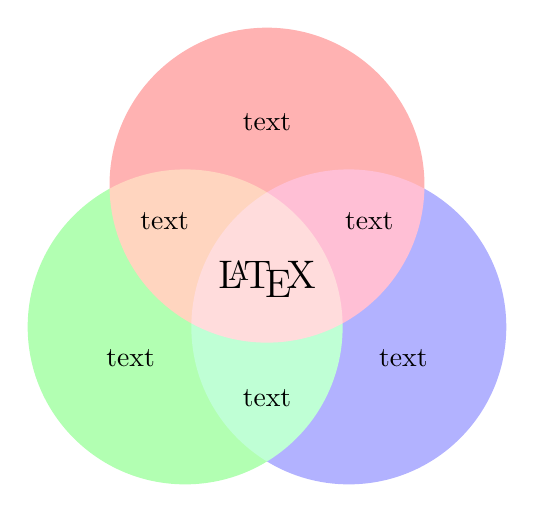
\begin{tikzpicture}
	\begin{scope}[blend group = soft light]
		\fill[red!30!white]   ( 90:1.2) circle (2);
		\fill[green!30!white] (210:1.2) circle (2);
		\fill[blue!30!white]  (330:1.2) circle (2);
	\end{scope}
	\node at ( 90:2)    {text};
	\node at ( 210:2)   {text};
	\node at ( 330:2)   {text};
	\node [font=\Large] {\LaTeX};
	\node at (150:1.5) {text};
	\node at (270:1.5) {text};
	\node at (30:1.5) {text};
\end{tikzpicture}
	
	\printbibliography
	
	% \appendix
	% \chapter{More Monticello Candidates}
	
\end{document}
